\section{Experiment}
\subsection{Setup}
\subsubsection{Point localization}

\begin{figure}[]
  \centering
  \begin{subfigure}[]{.2\textwidth}
    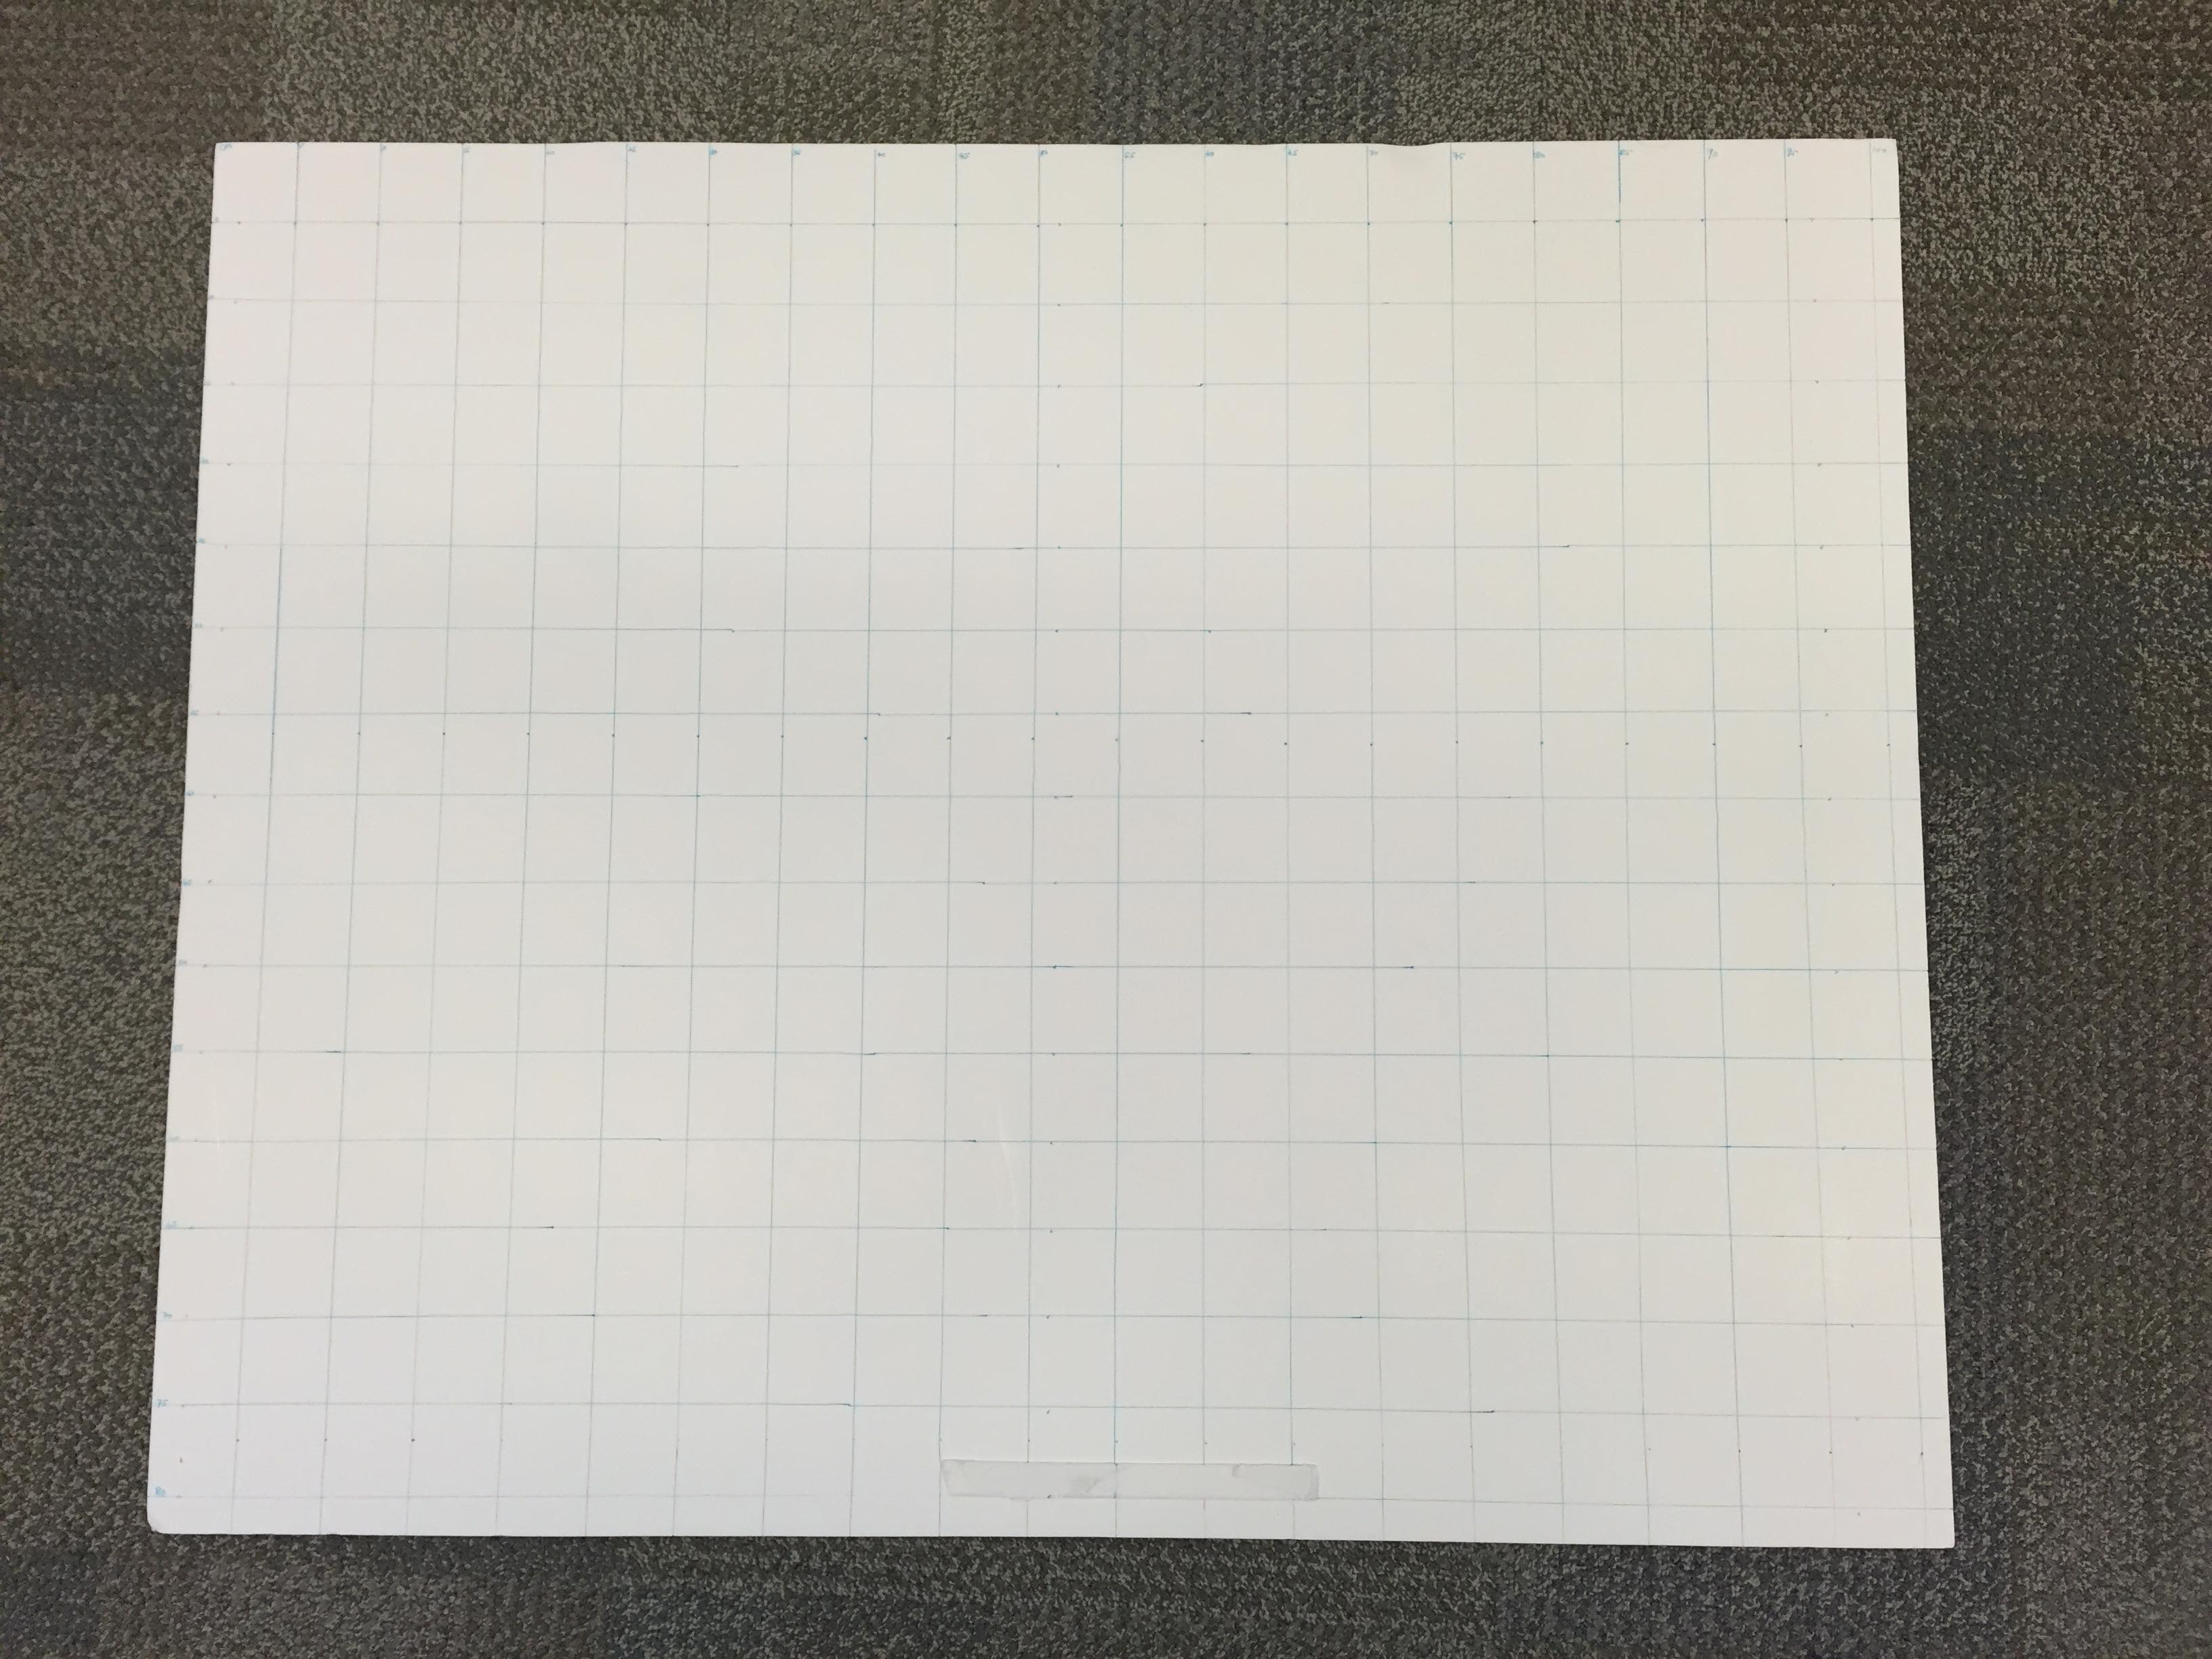
\includegraphics[width=\textwidth]{setup_1.JPG}
    \caption{1 meter by 1 meter grid}
  \end{subfigure}
  \begin{subfigure}[]{.2\textwidth}
    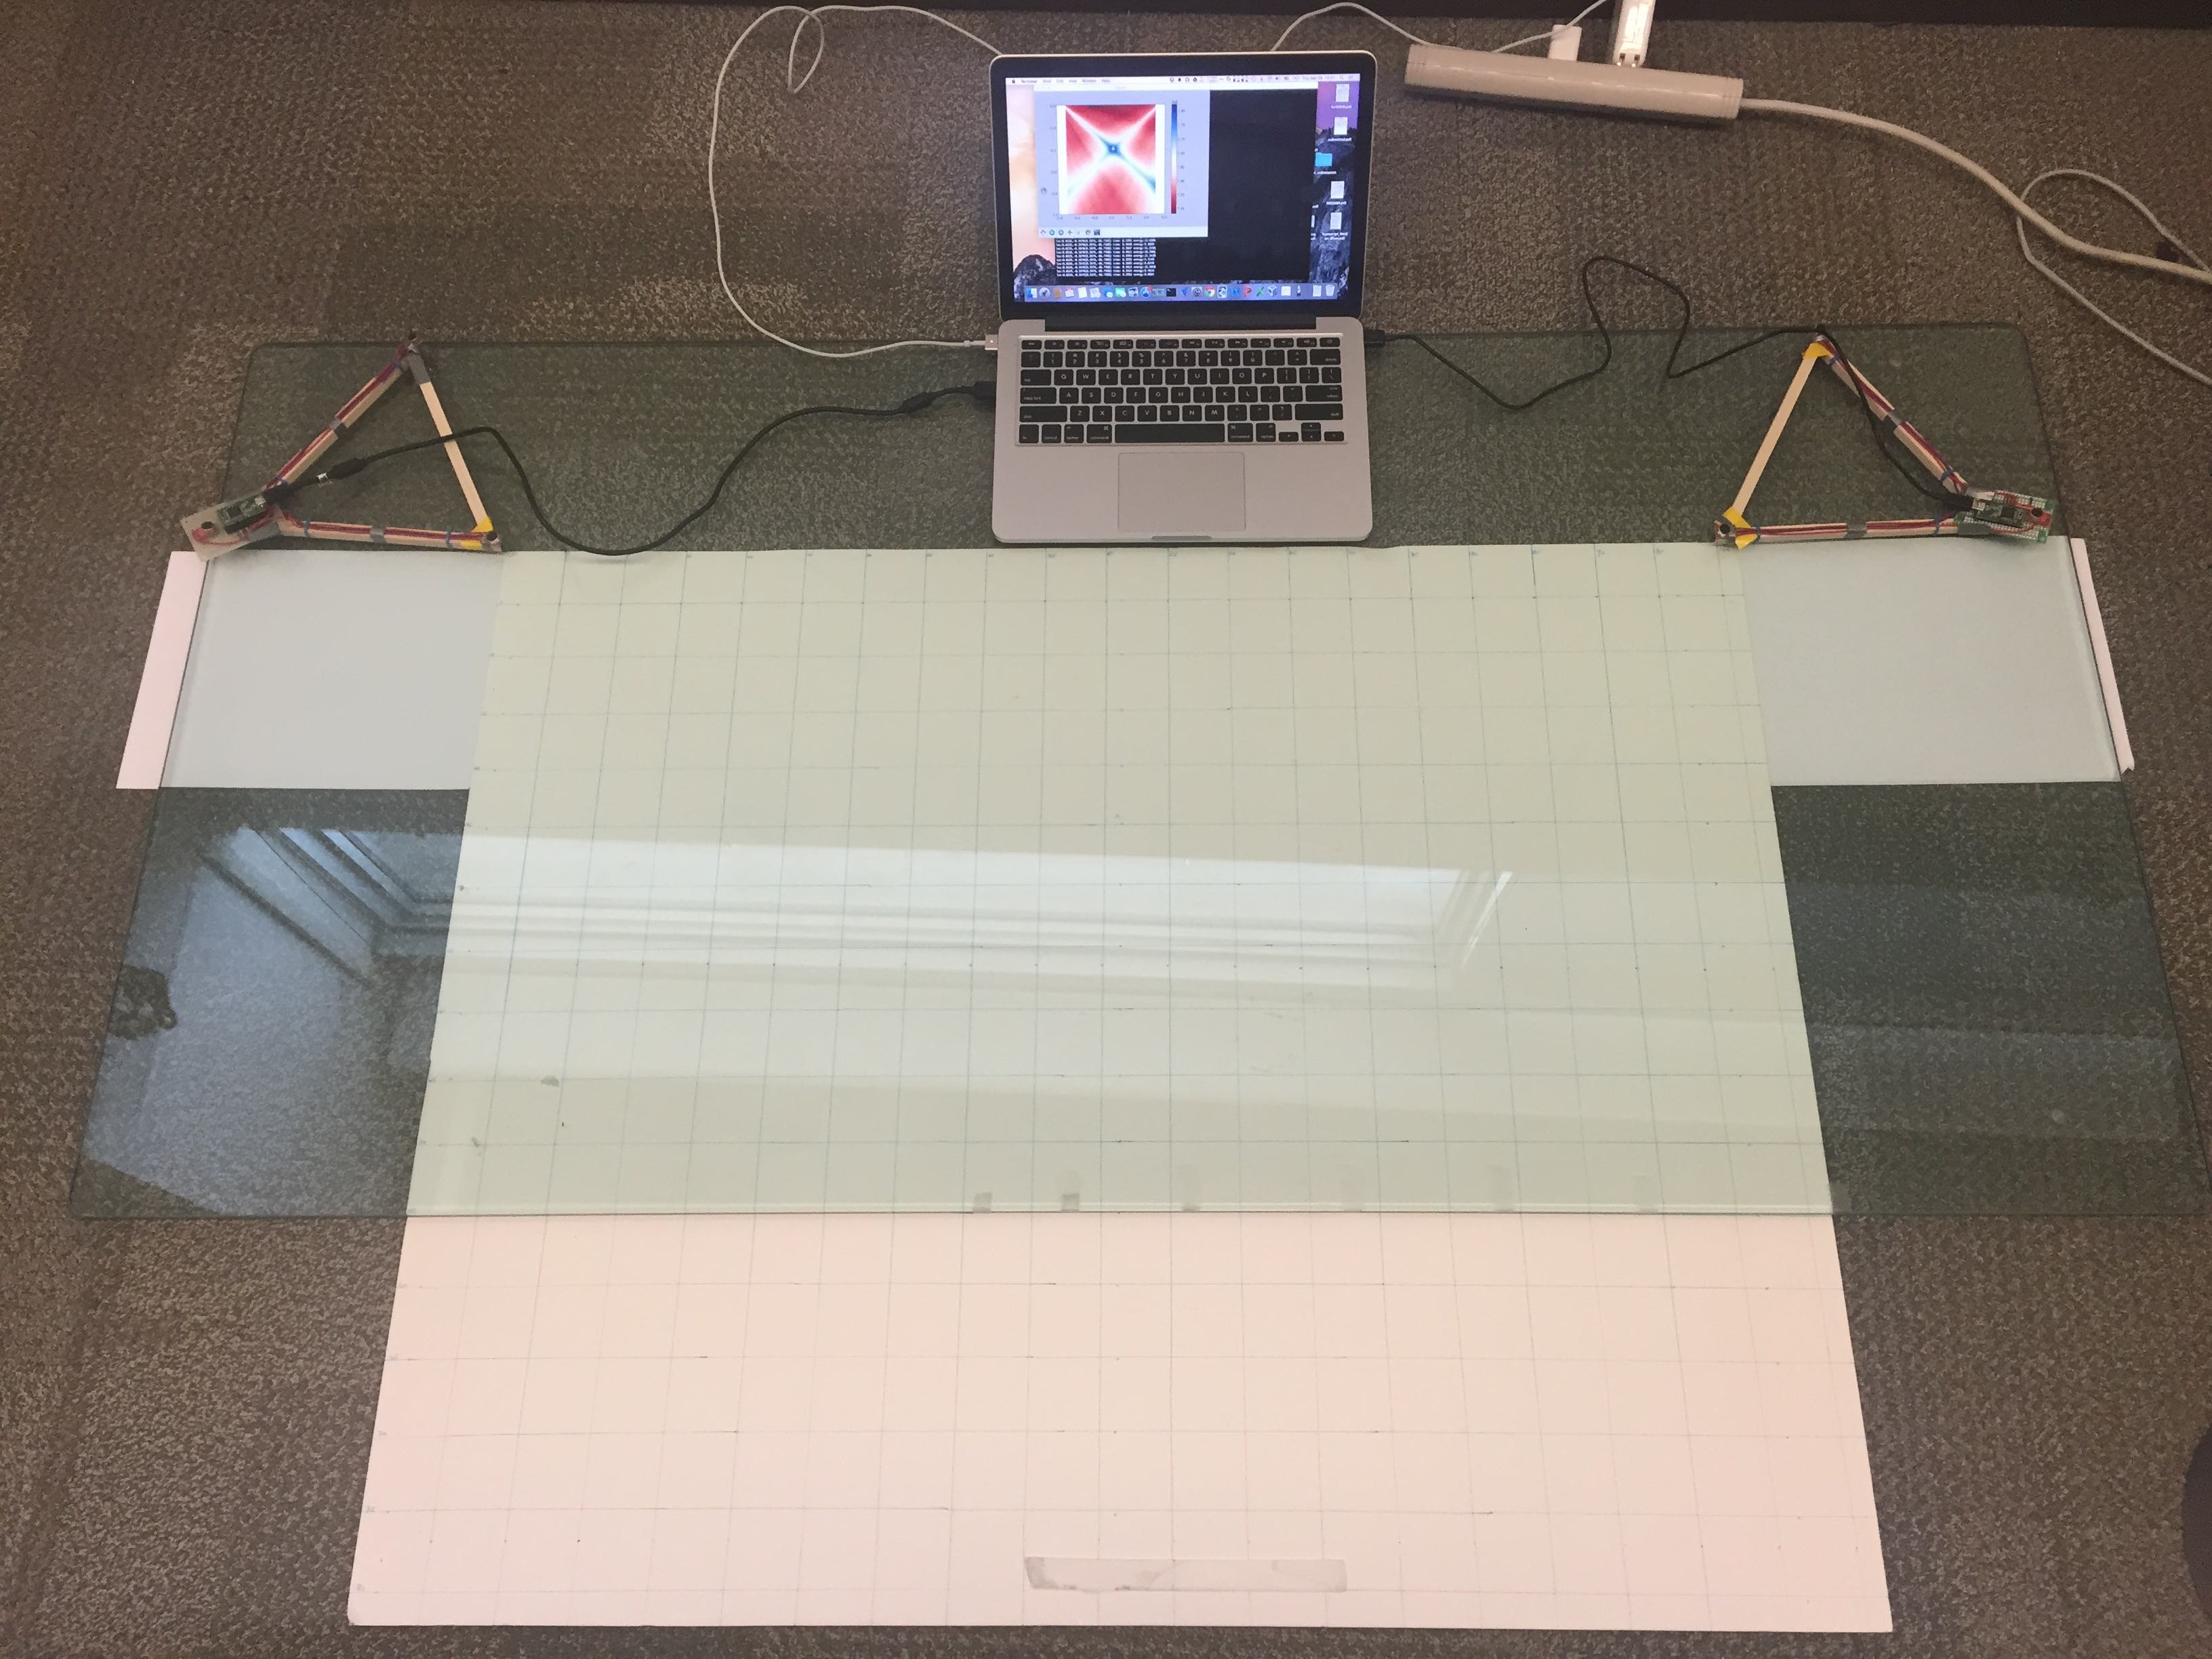
\includegraphics[width=\textwidth]{setup_2.JPG}
    \caption{array placement}
  \end{subfigure}
  \caption{Setup for localization accuracy testing}
  \label{fig:setup_point}
\end{figure}

To test localization accuracy, an one meter by one meter grid was set up and the arrays are placed at the top left and top right corners of the grid. Fig~\ref{fig:setup_point} shows a picture of the setup. A total of $32$ positions are chosen uniformly in this region where microphone data is recorded.

\subsubsection{Movement tracking}
To test how well the arrays track movement, we mounted a rotating disk $40$ centimeter in diameter onto the grid at $(x=0, y=-0.3)$. Fig~\ref{fig:setup_circle} shows a picture of the sestup. A sound source is placed on the edge of rotating disk and the arrays localizes the sound source as it rotates in a circle. In this experiment, we tested how accuracy changes with:
\begin{itemize}
\item different window sizes
\item different audio sources
\item different movement tracking filters
\item different movement speeds
\end{itemize}

To test how different sound sources impact localization quality, we conducted three experiments on the same movement track with three different sound sources:

\begin{description}[\IEEEsetlabelwidth{long a label}\IEEEusemathlabelsep]

\item[White Noise] A recording of white noise.

\item[Music A] A music that has normal audio amplitude throughout experiment period was chosen. "Honest Eyes" by Black Tide was the music used.

\item[Music B] A music with intermittent low amplitude sections was chosen. "Canon" was the music used.

\end{description} 

To test how sound source movement speed affects localization quality, each of three experiments were conducted at two different speeds:
\begin{description}
\item[Normal] An angular speed of $0.5$ rad/s was maintained, which translates to linear speed of $10$ cm/s.
\item[Fast] An angular speed of $1.0$ rad/s was maintained, which translates to linear speed of $20$ cm/s.
\end{description}

For each experiment conducted, two different movement filters are tests:
\begin{description}[\IEEEsetlabelwidth{Very long label}\IEEEusemathlabelsep]
\item[Averaging filter] localization for past $0.5$ seconds are averaged and outputed as current estimate.
\item[Kalman filter] A 2nd order Kalman filtering is used.
\end{description}

\subsection{Results}
\subsubsection{Point localization}

To test how accuracy varies with window size, the algorithm is fed with recorded microphone data with different segment length. Fig~\ref{fig:accuracy_vs_window} shows how accuracy changes with window length for three GCC algorithms. The error lowers as window size increases and plataeus after window size exceeds around $10$ milli-second. The lowest error achieved is $2.53$ centimeters. It is achieved when window size is set to 12 millisecond and GCC\_PHAT is used for TDOA estimation.

Although accuracy improves with window length, the calculation time also increases with window length. The part of calculation that depends on window length is using cross correlation to estimate TDOA. cross correlation can be calculated with FFT and the runtime is of order $O(N\log N)$. We measured how the computation time varies with window length and Figure~\ref{fig:speed_vs_window} shows the result. The runtime increases approximately linearly in the window size region of interest.

We also calculated the localization error for each tested point in the region. Figure~\ref{fig:error_distribution} shows a heatmap of the error distribution inside the grid. The error is below $3$ cm for most areas inside the region. There is one error spike in the mid-left region and we contribute this to audio source placecment error becuase the error is fairly low and consistent around that spike region.

\begin{figure}[]
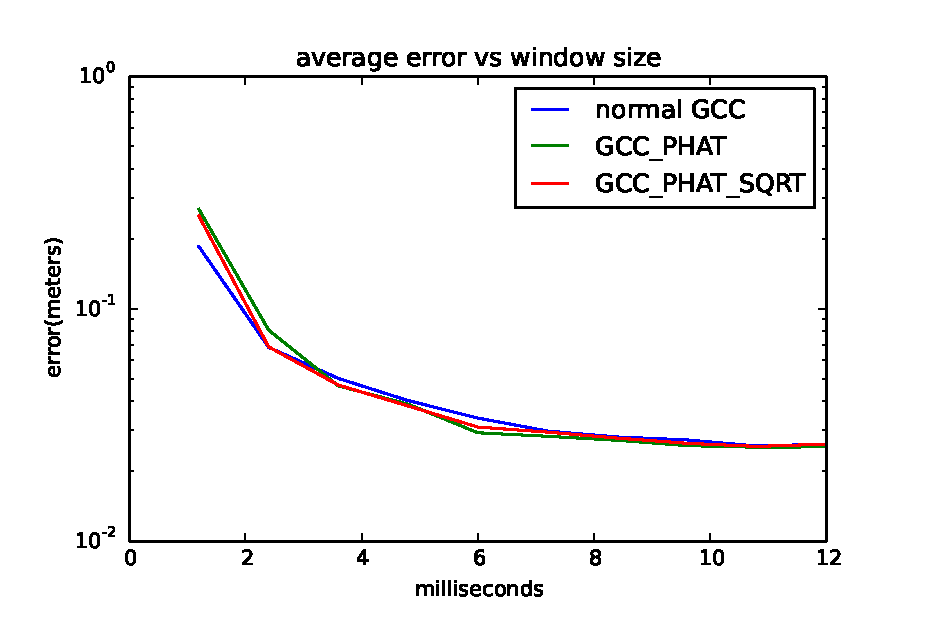
\includegraphics[width=0.5\textwidth]{average_error_window_size.eps}
\caption{accuracy versus window size}
\label{fig:accuracy_vs_window}
\end{figure}

\begin{figure}[]
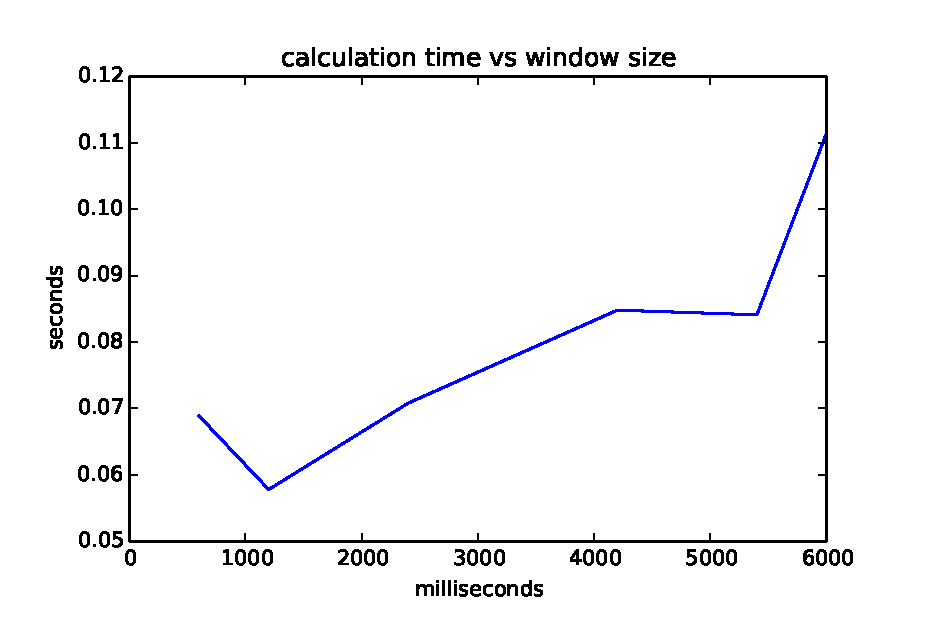
\includegraphics[width=0.5\textwidth]{calculation_time.eps}
\caption{speed versus window size}
\label{fig:speed_vs_window}
\end{figure}


\begin{figure}[]
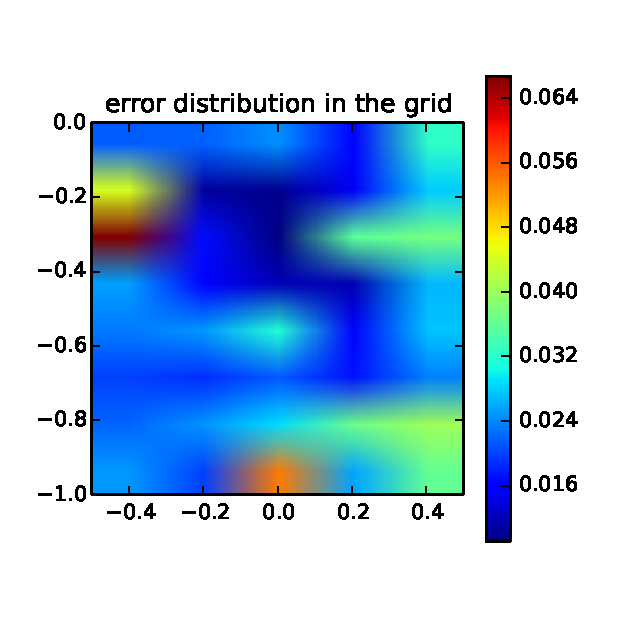
\includegraphics[width=0.5\textwidth]{error_distribution.eps}
\caption{error distribution in the grid}
\label{fig:error_distribution}
\end{figure}

\begin{figure}[]
  \centering
  \begin{subfigure}[]{.2\textwidth}
    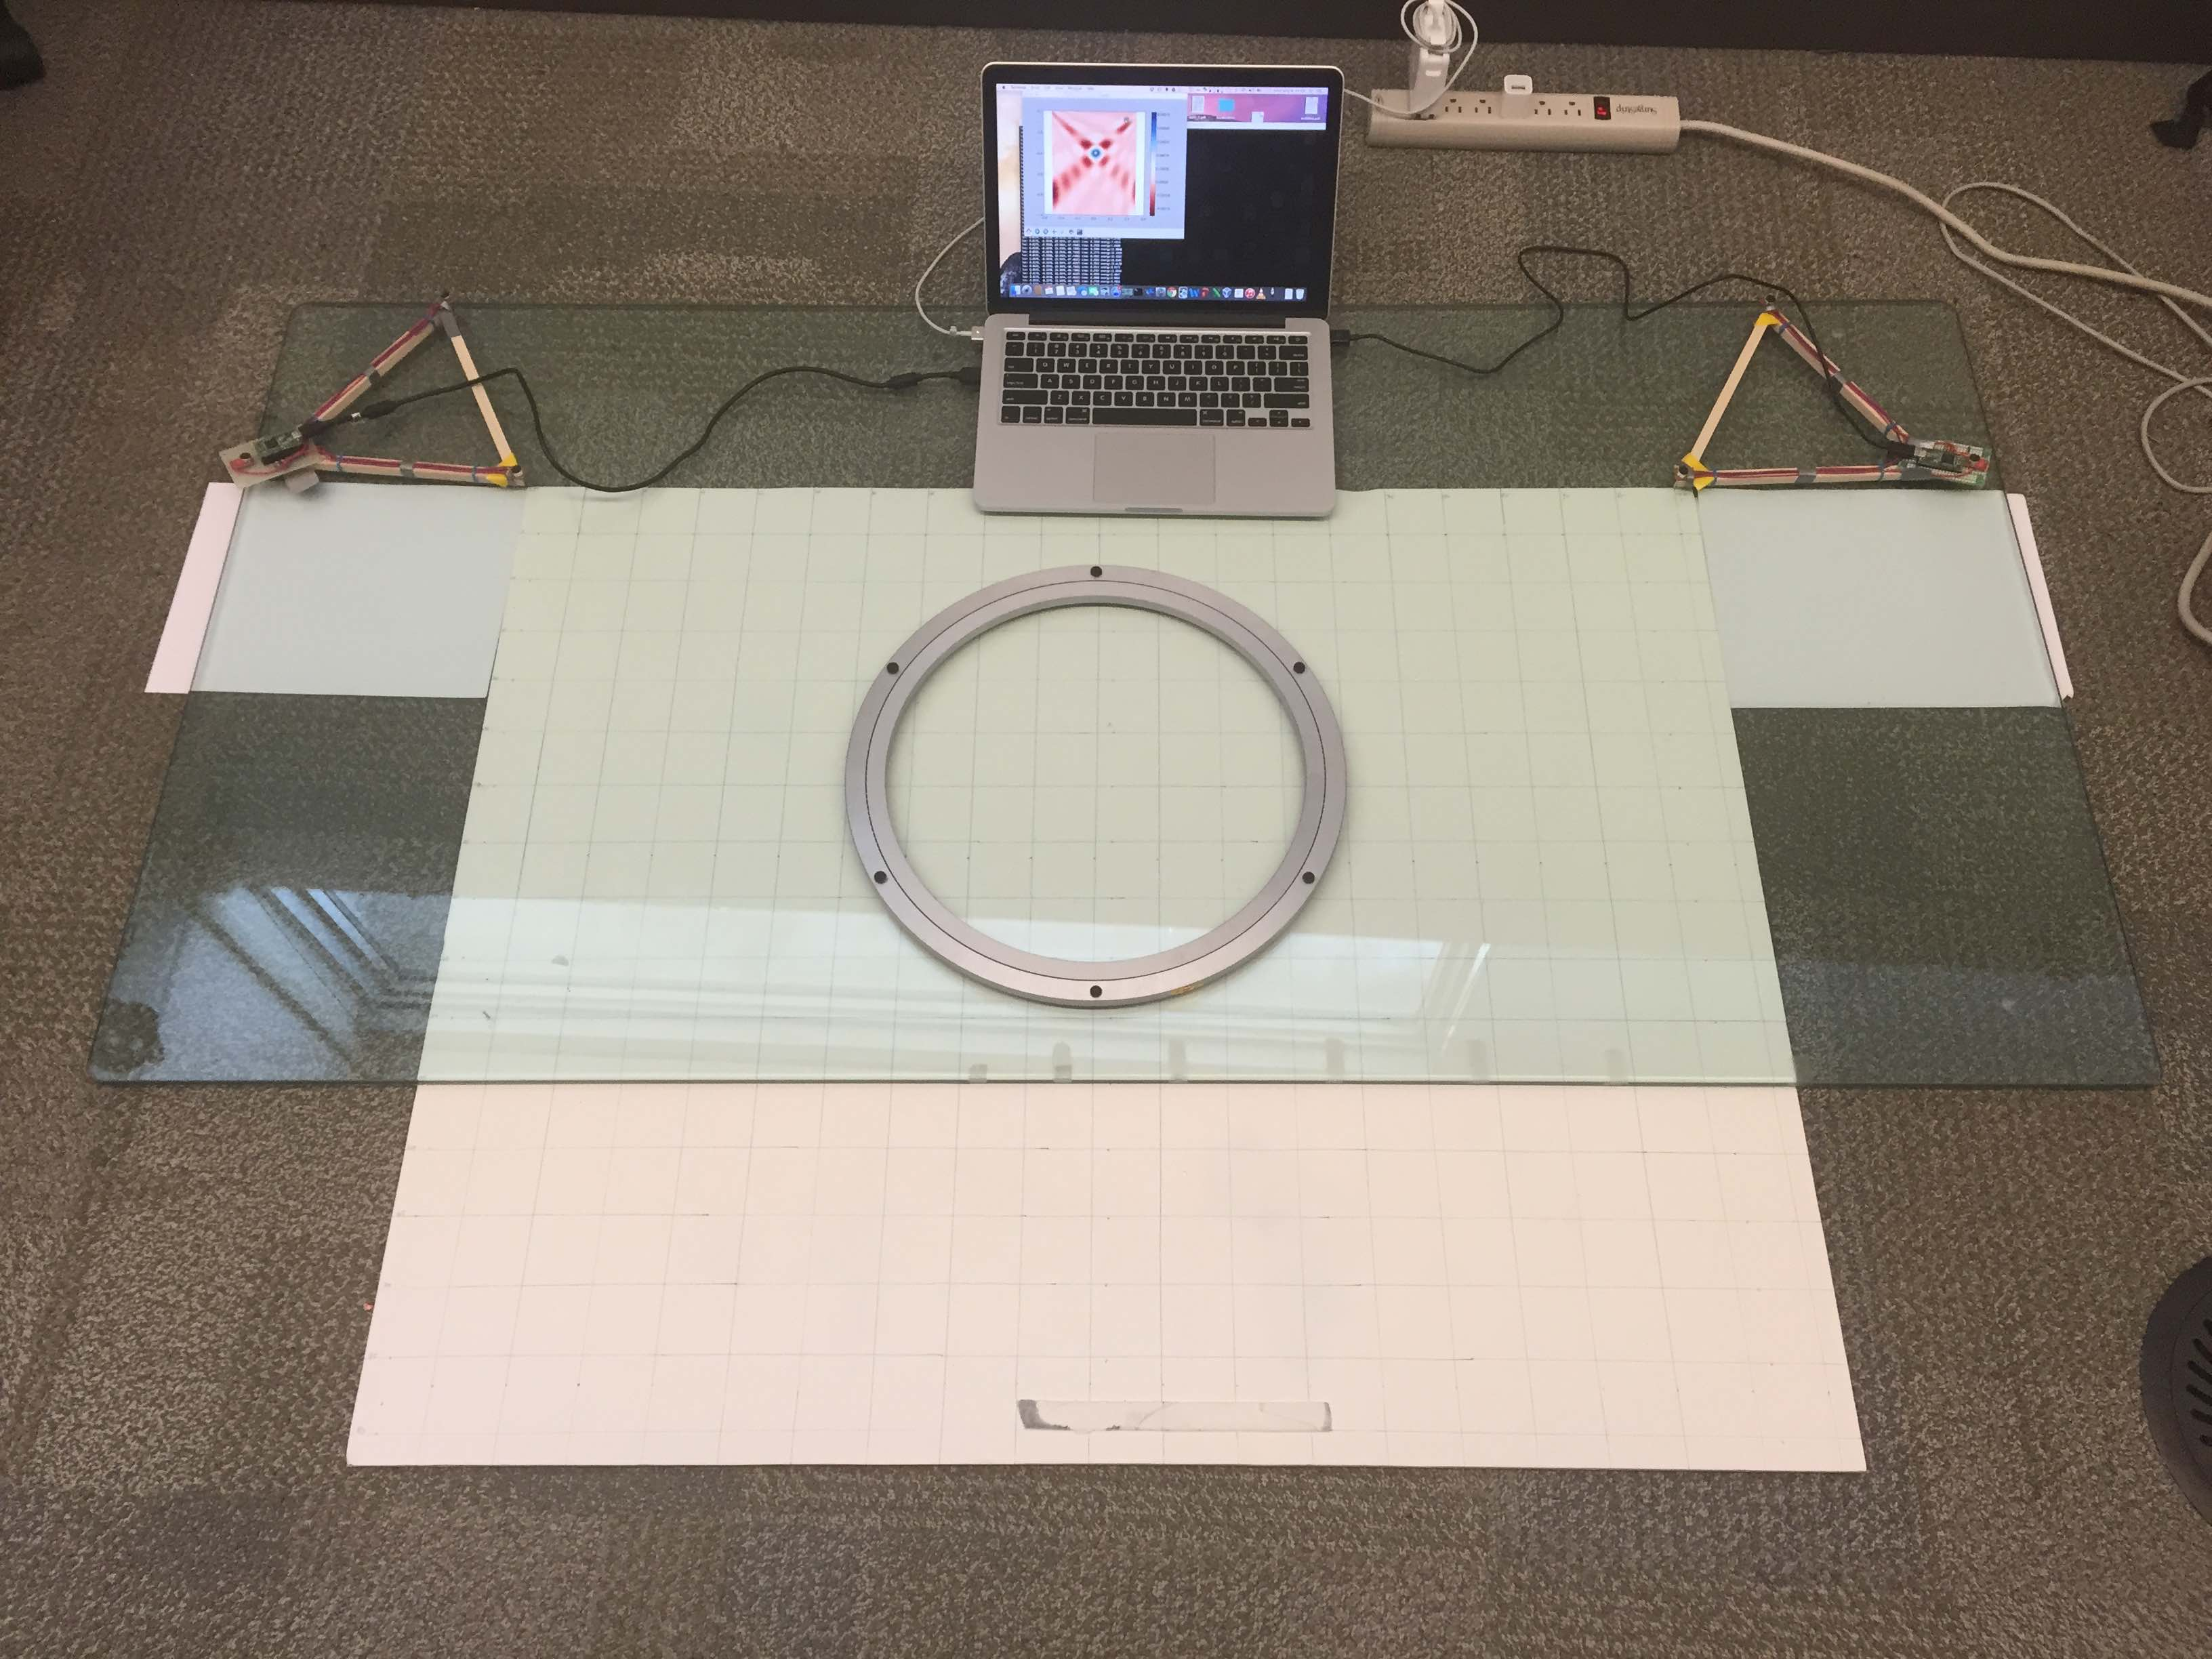
\includegraphics[width=\textwidth]{setup_ring.JPG}
  \end{subfigure}
  \begin{subfigure}[]{.2\textwidth}
    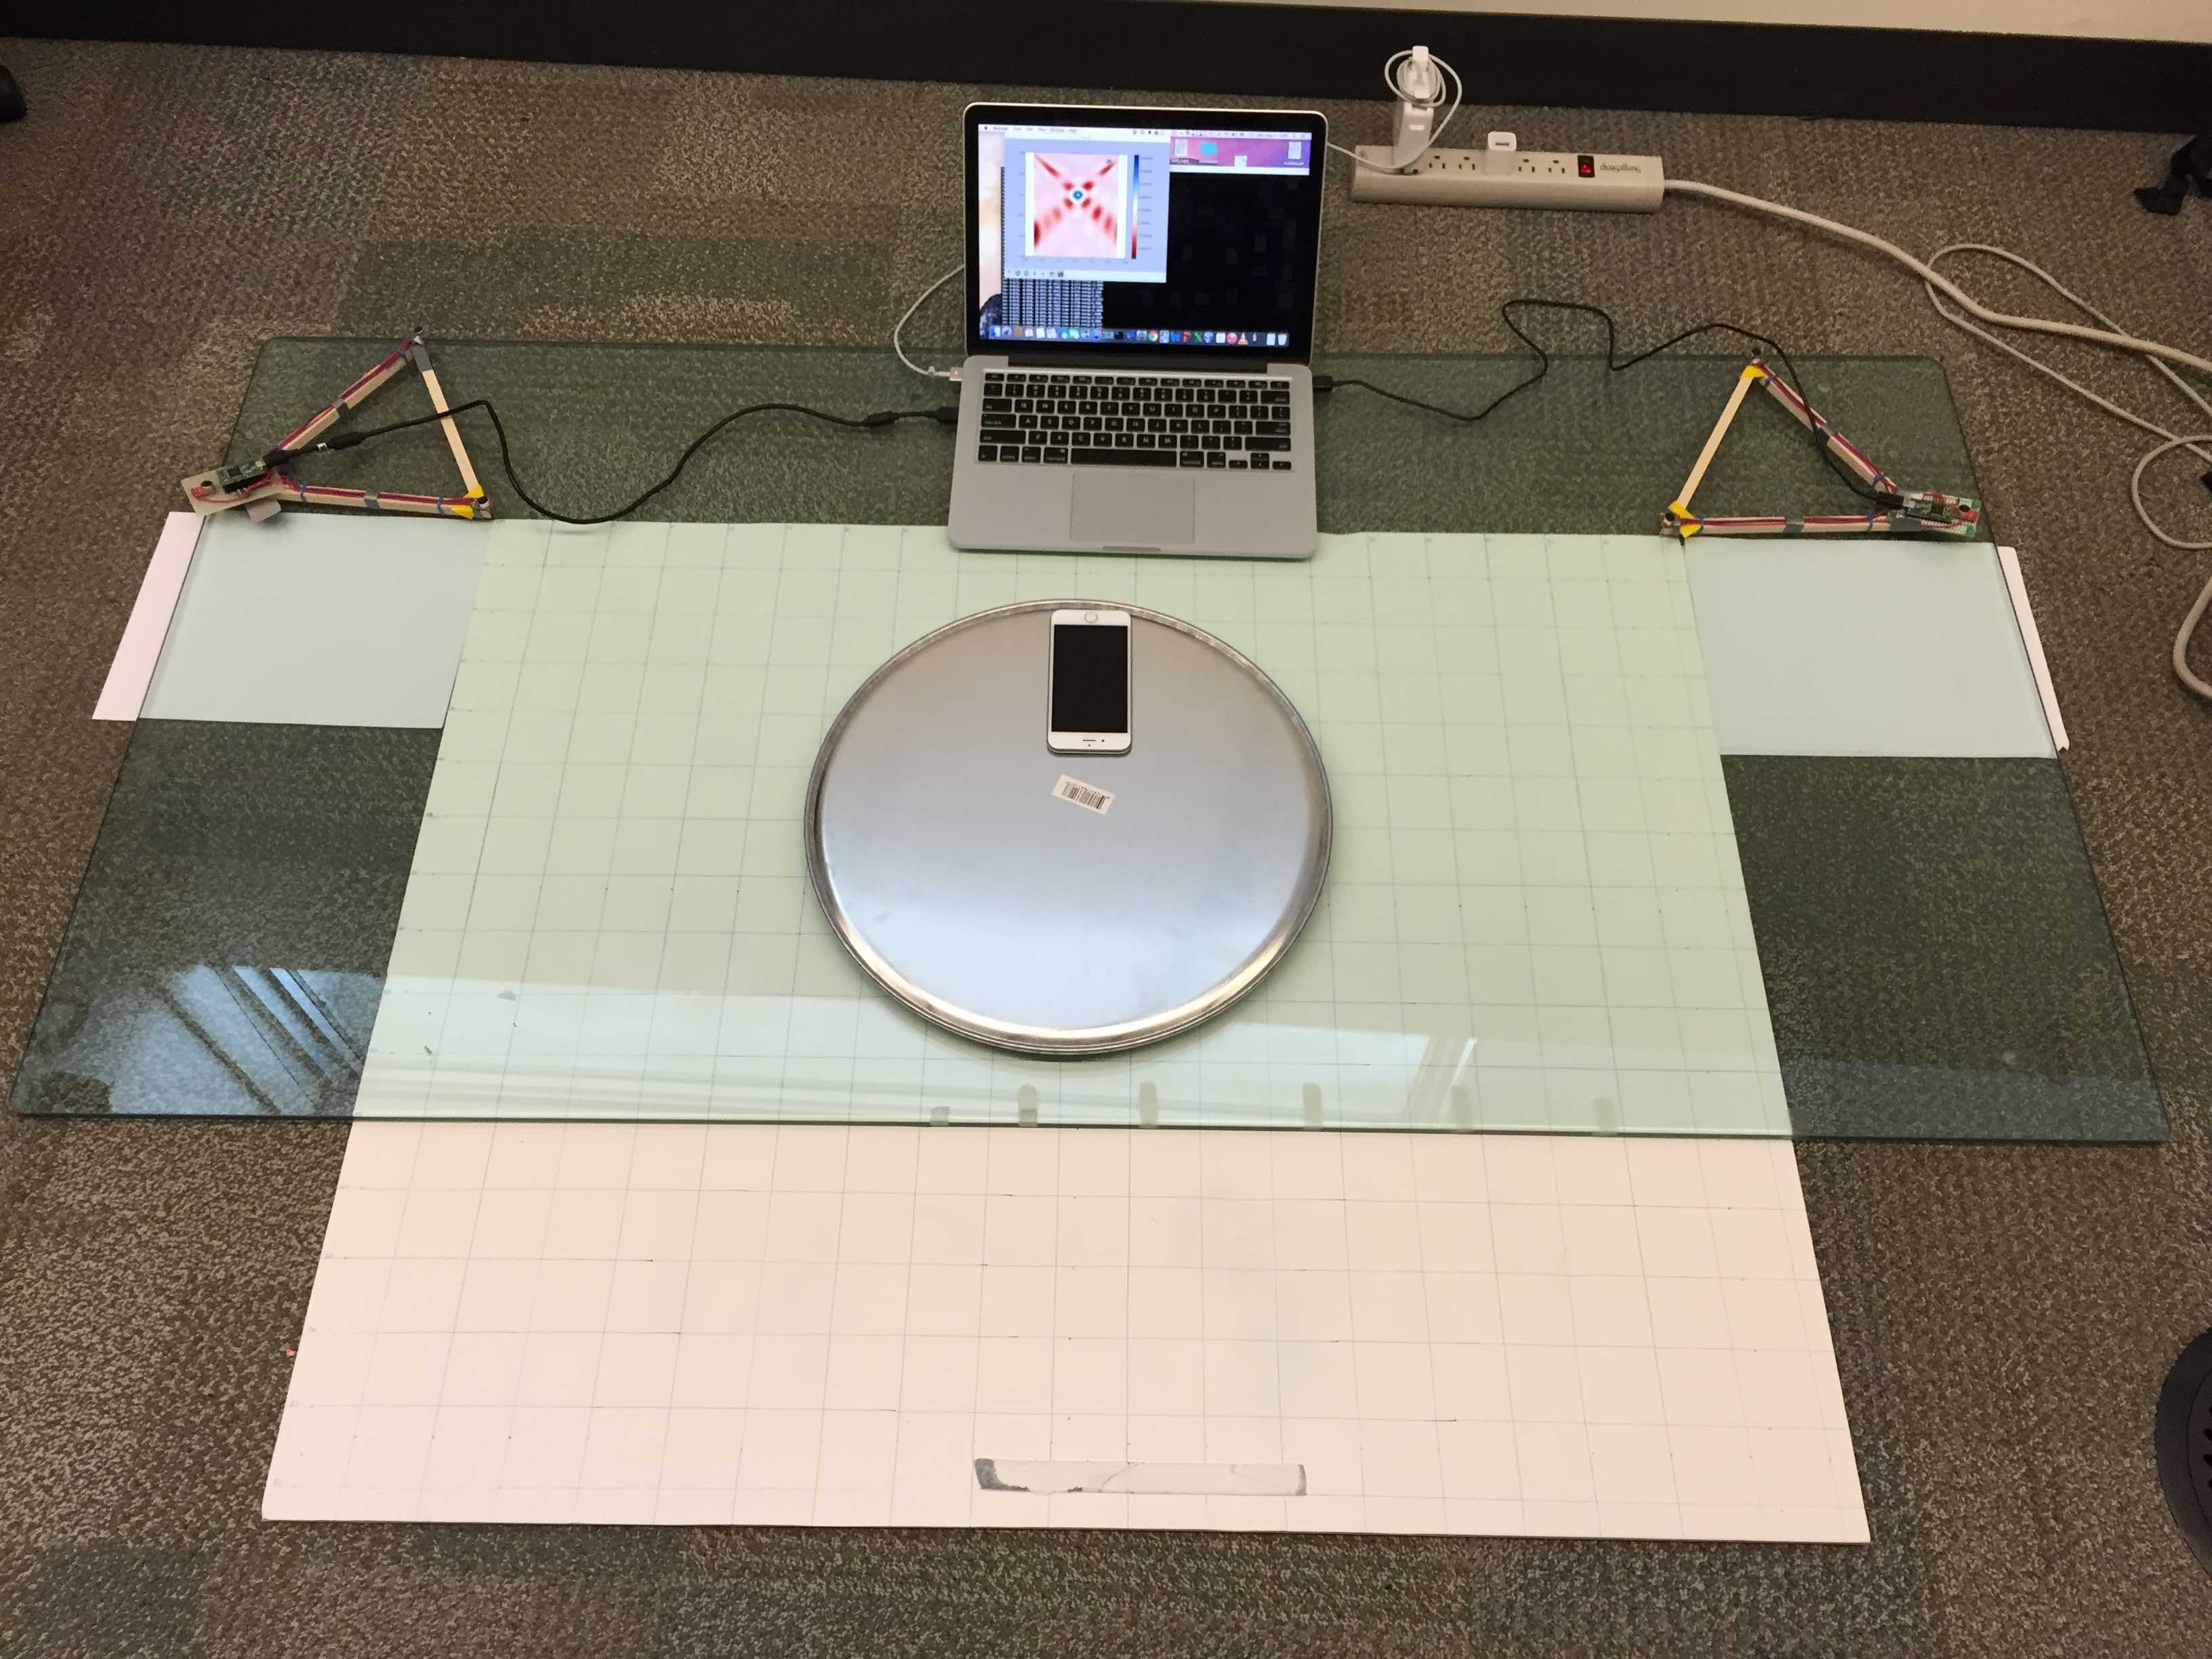
\includegraphics[width=\textwidth]{setup_rotating_disk.JPG}
  \end{subfigure}
  \caption{Setup for circle movement localization}
  \label{fig:setup_circle}
\end{figure}


\begin{figure*}[]
\centering
  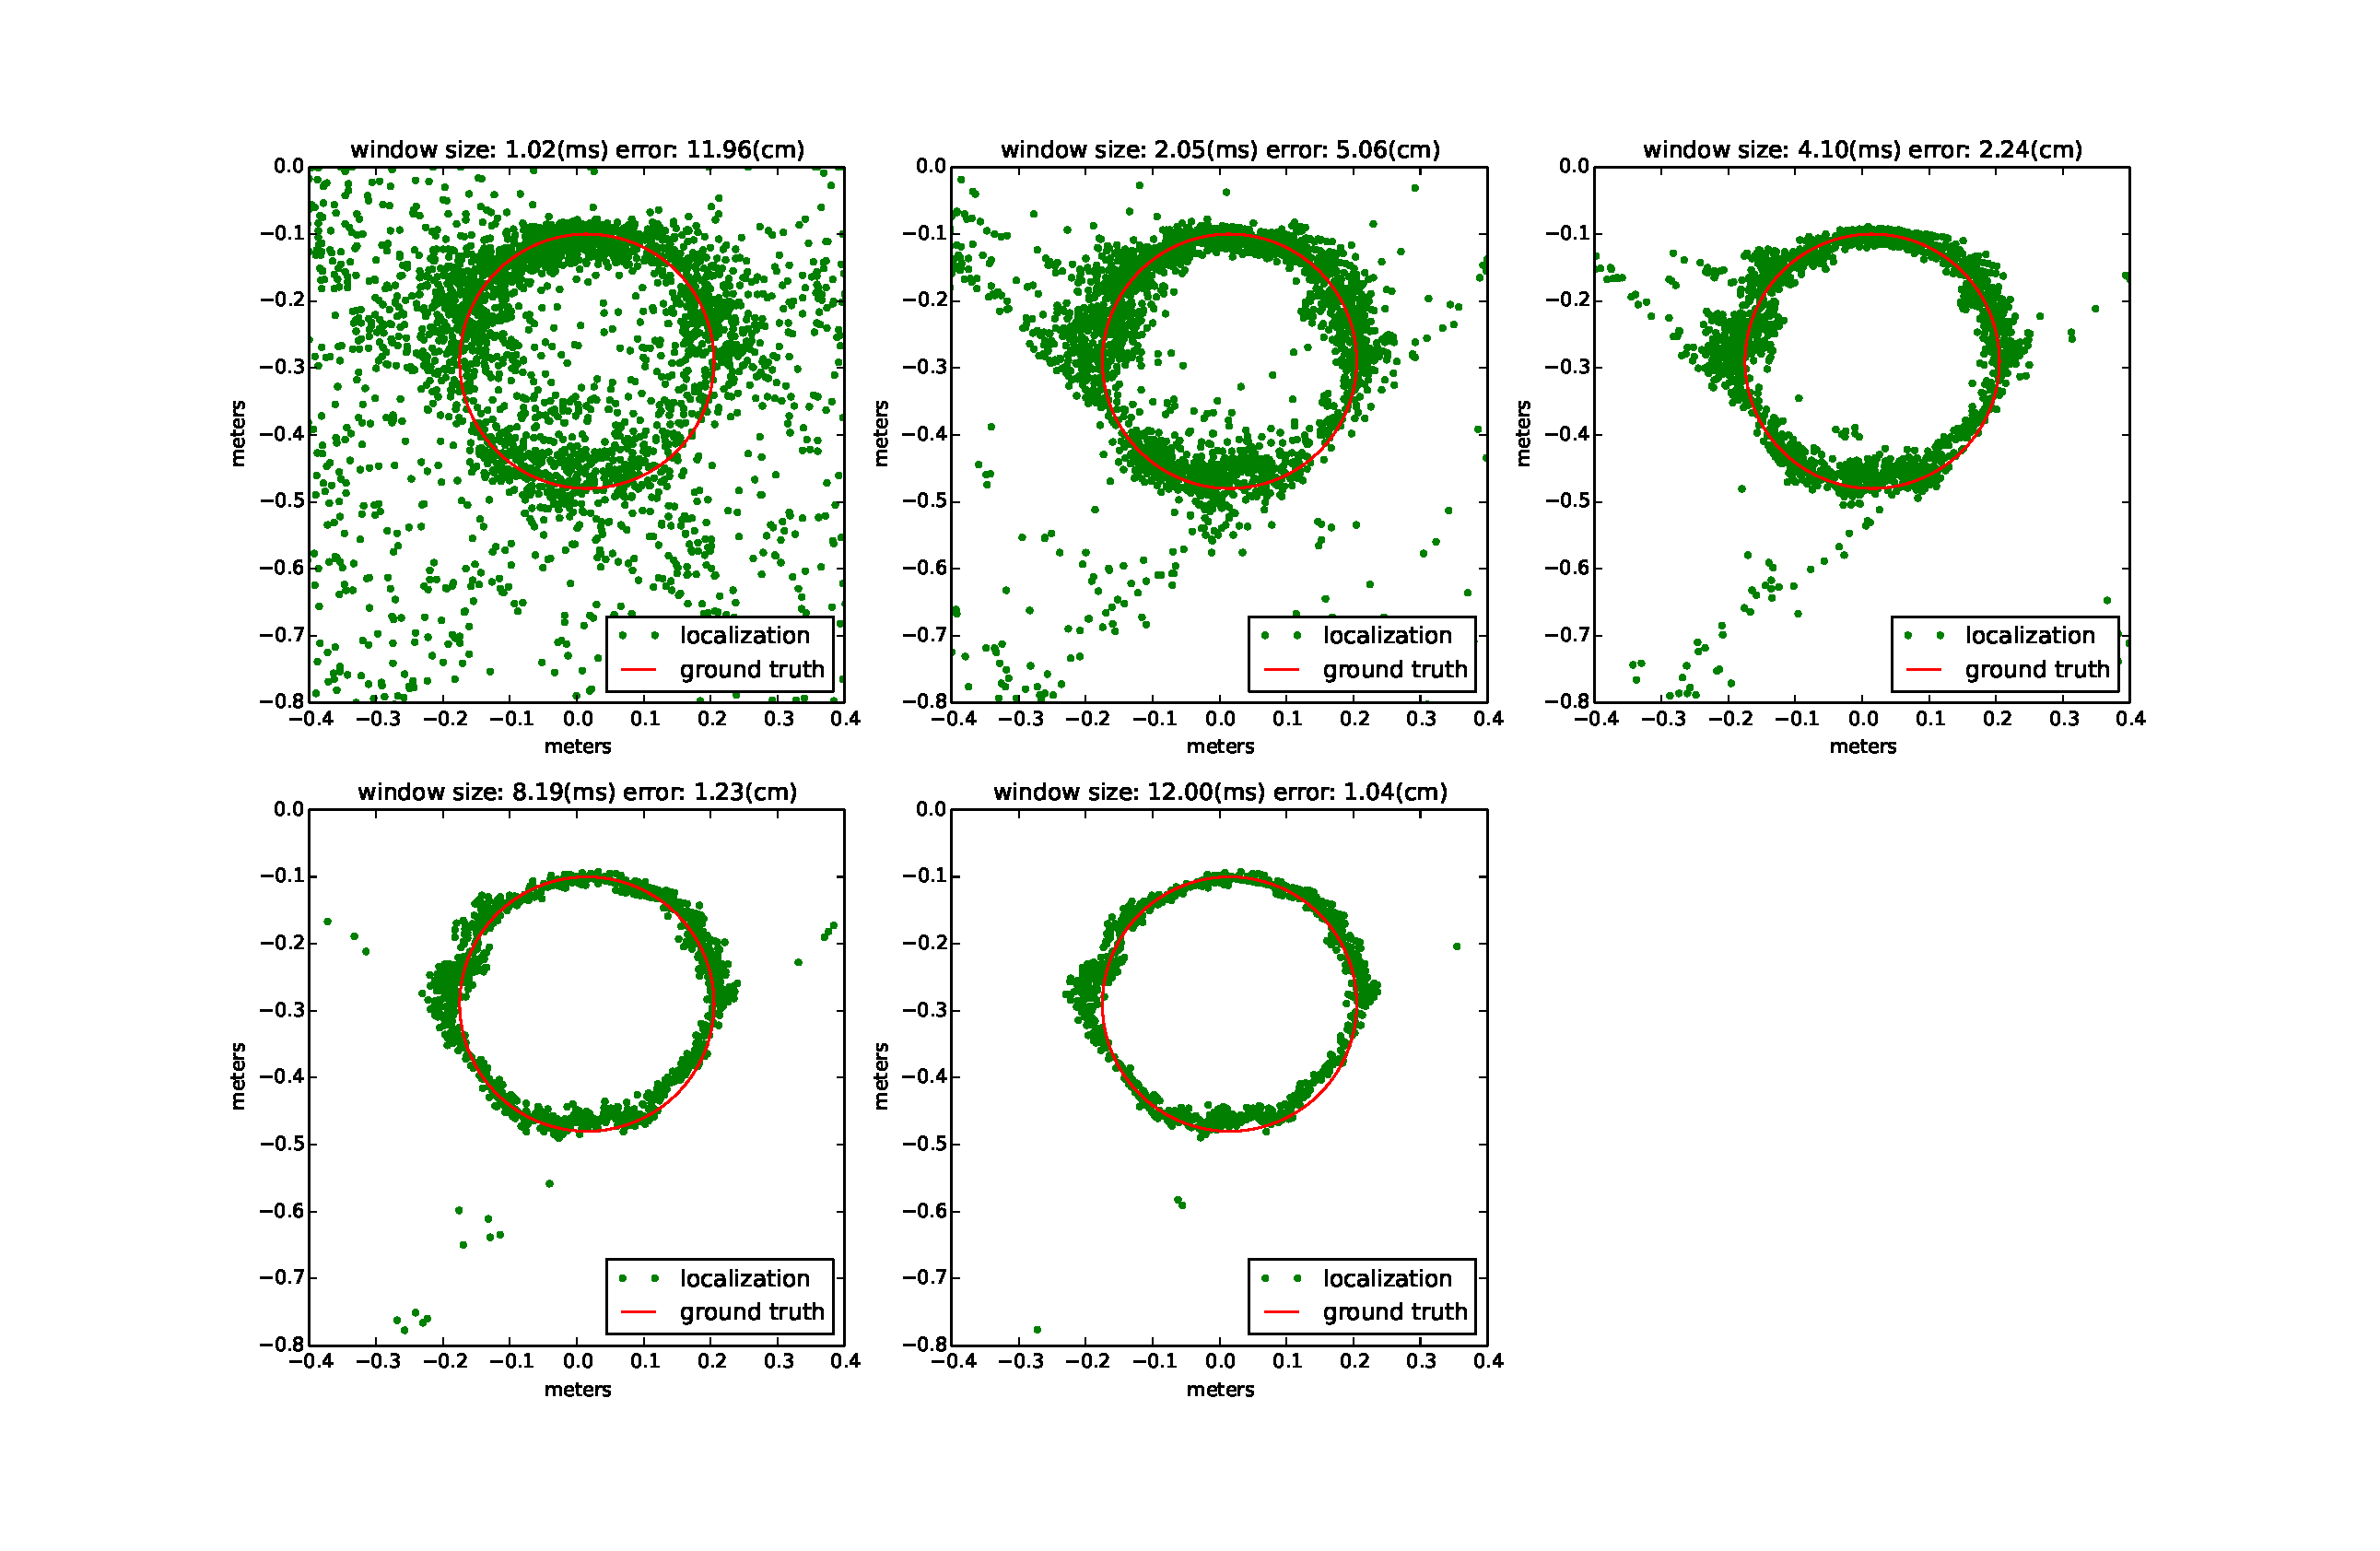
\includegraphics[width=\textwidth]{trace_window_size_movement.eps}
\caption{Localization quality versus window size}\label{fig:wn}
\label{fig:trace_win_circle}
\end{figure*}

\begin{figure}[]
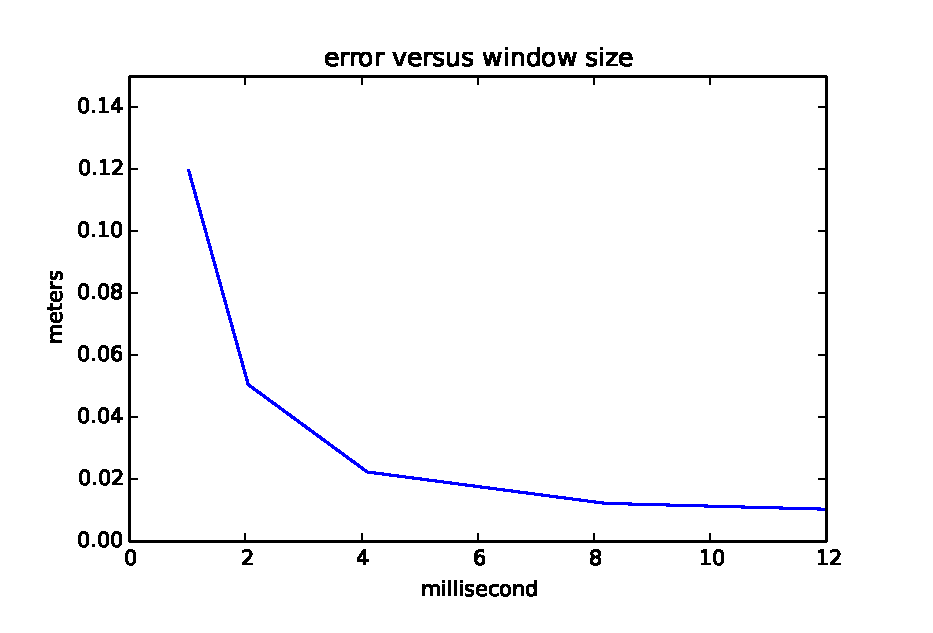
\includegraphics[width=0.5\textwidth]{error_window_size_movement.eps}
\caption{Localization error versus window size}
\label{fig:err_win_circle}
\end{figure}

\subsubsection{Movement tracking}

Fig~\ref{fig:err_win_circle} gives an intuitive representation of how accuracy changes with window size. When window size is small($1.02$ millisecond), the audio does not contain enough information to reliably estimate TDOA. The localization is noisy. As window size increases, the localization converges to the shape of ground truth circle. Fig~\ref{fig:err_win_circle} shows how the error changes with window size. The general trend is similar to that in point localization case. The error decreases as window size increases and plateaus after window size exceeds around $10$ milliseconds.

\begin{figure*}[]
\centering
\begin{subfigure}[]{1.0\textwidth}
  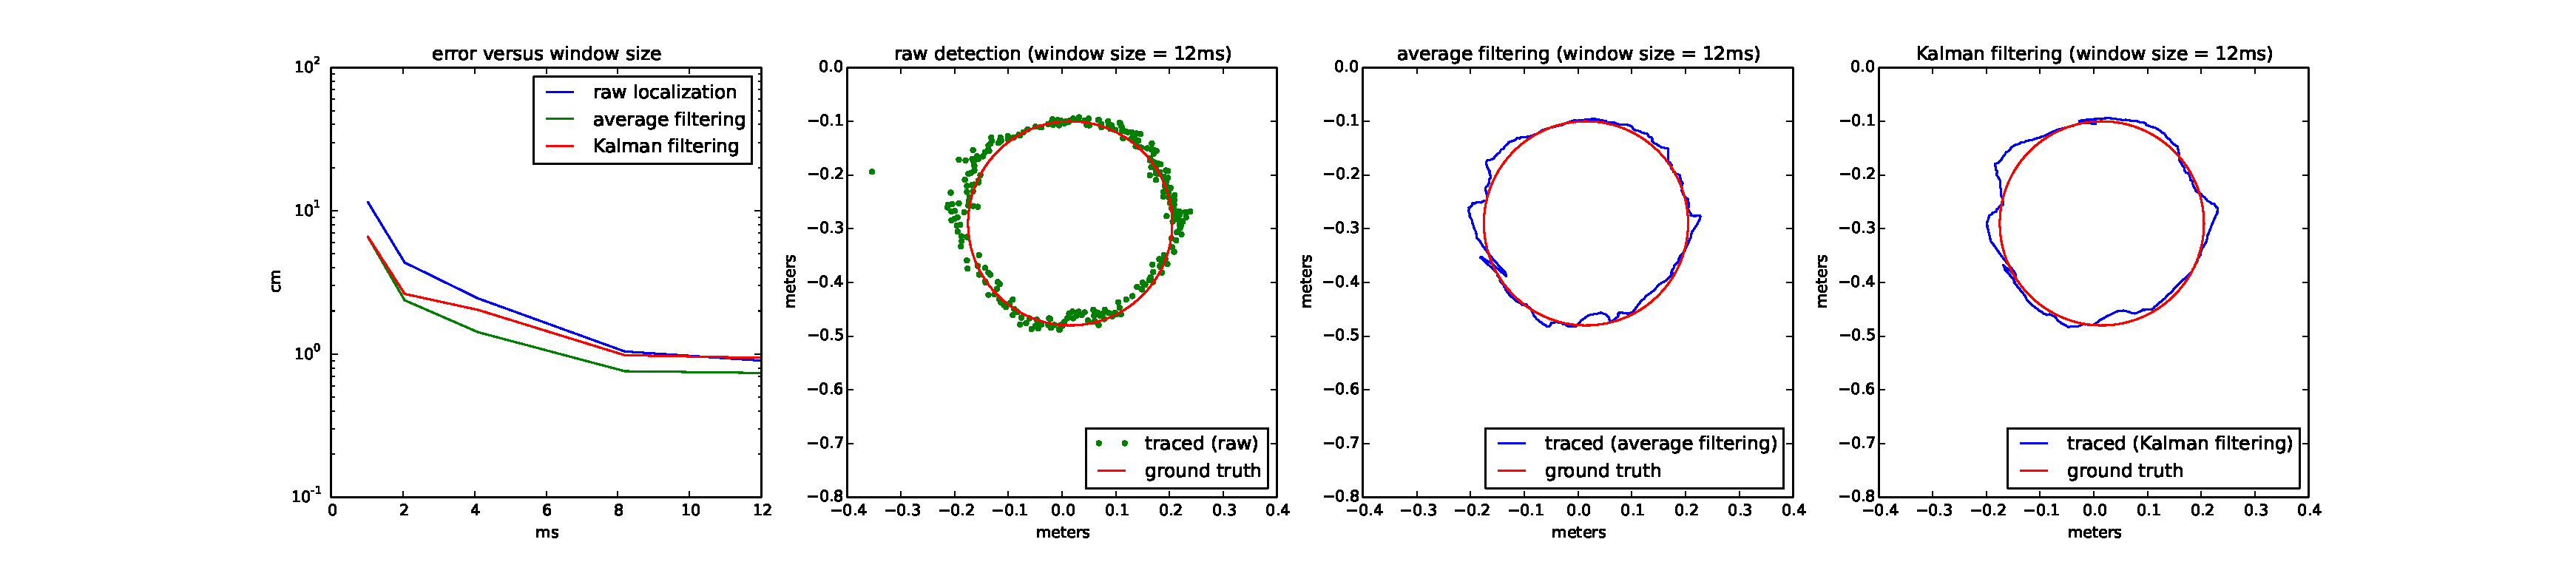
\includegraphics[width=1.0\textwidth]{trace_output_circle_wnn.eps}
  \caption{white noise}
  \label{fig:circle_wnn}
\end{subfigure}
\begin{subfigure}[]{1.0\textwidth}
  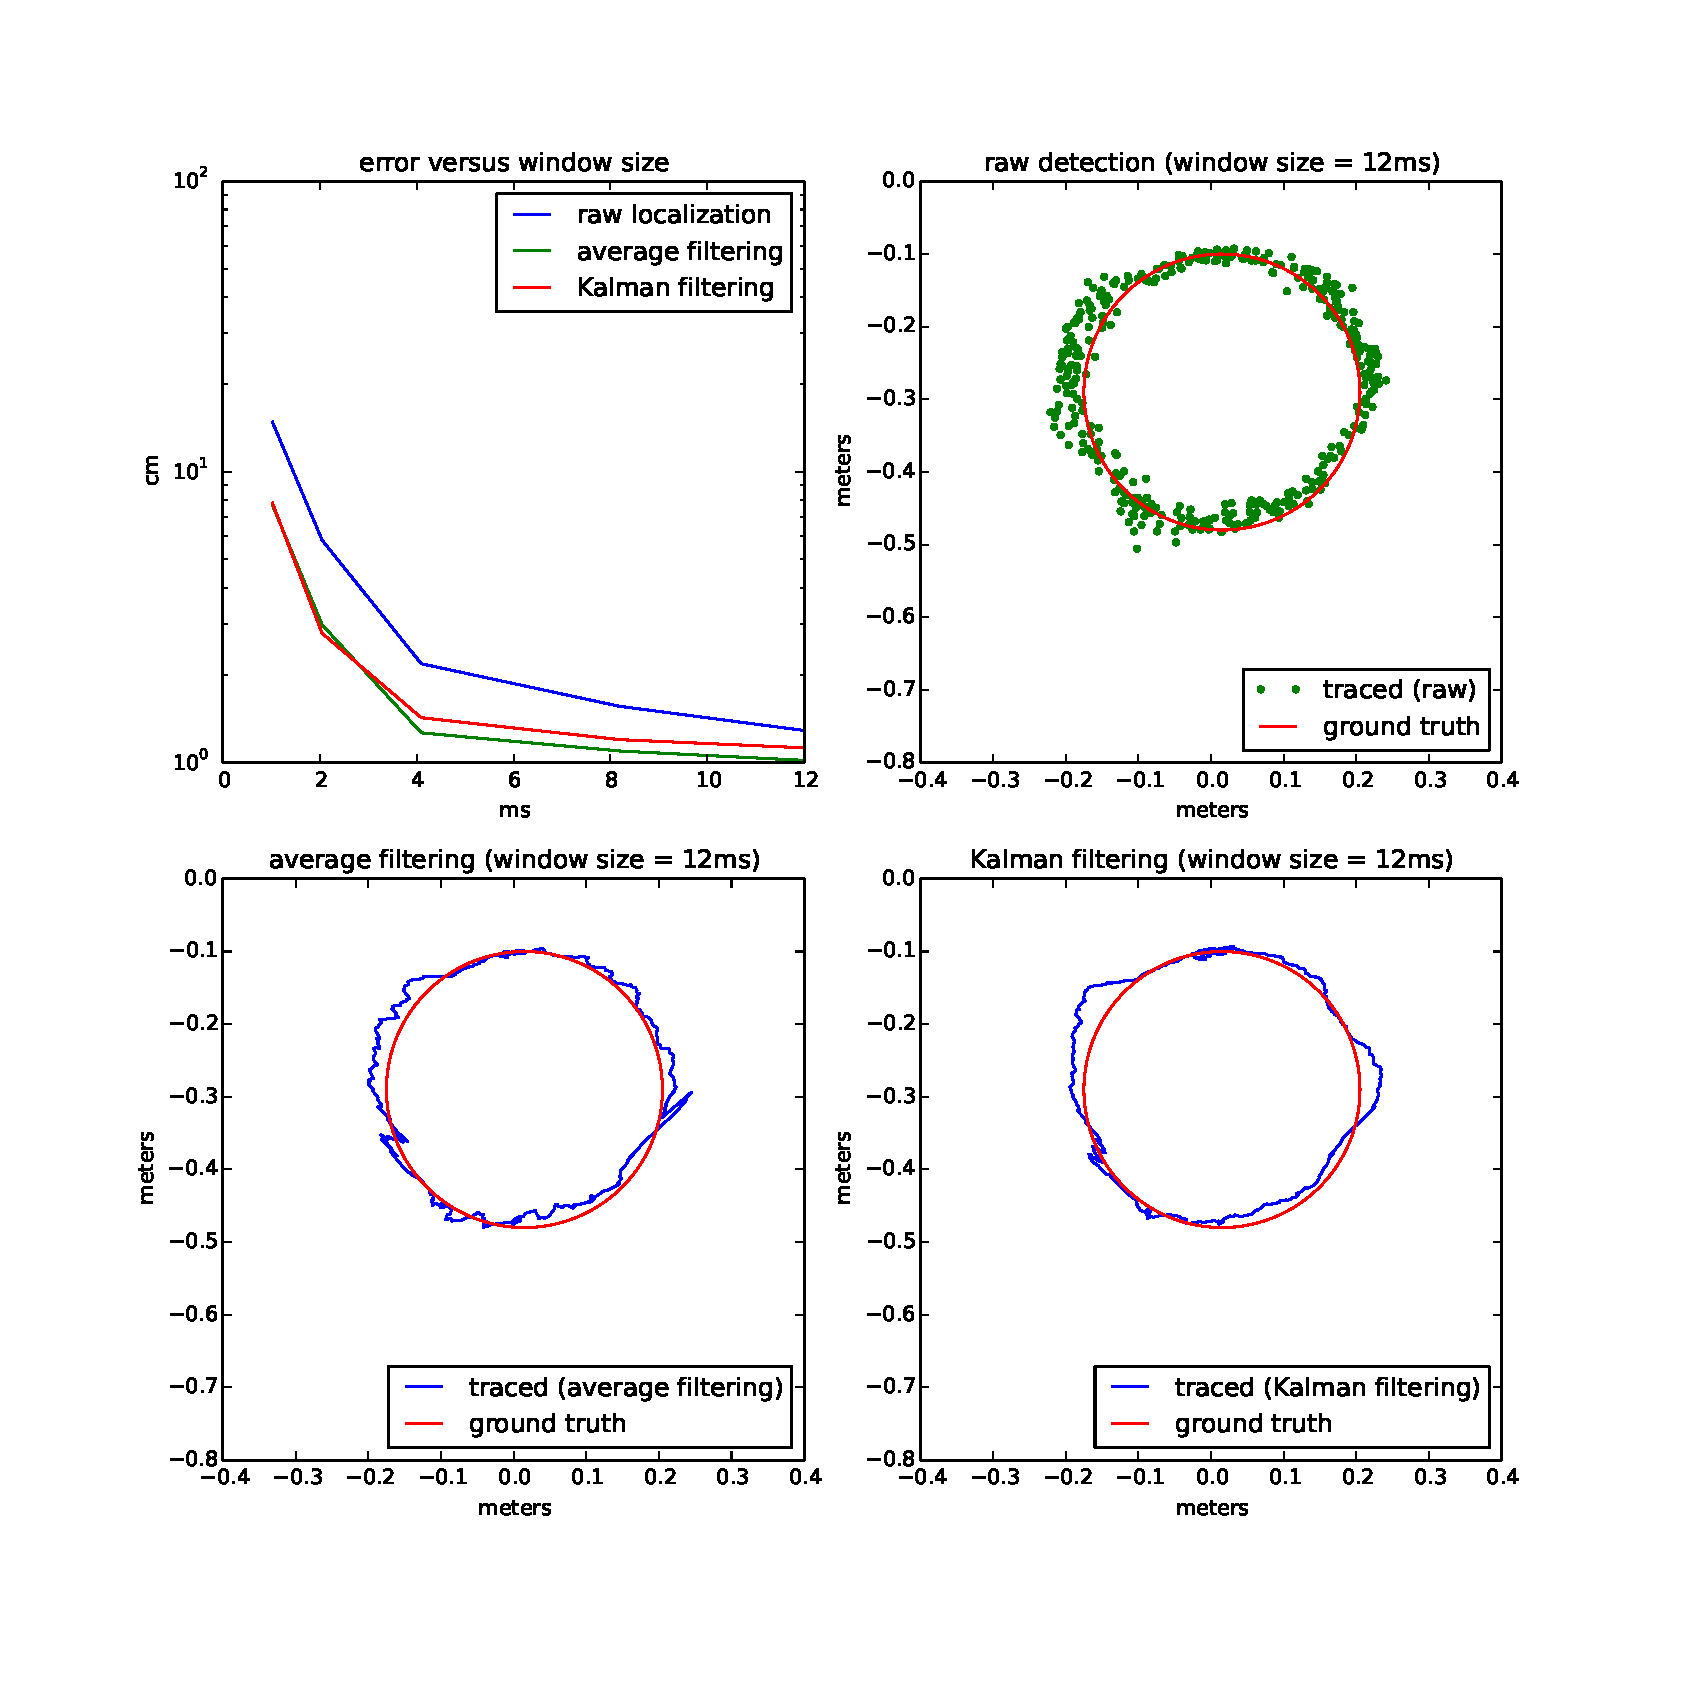
\includegraphics[width=\textwidth]{trace_output_circle_man.eps}
  \caption{music A}
  \label{fig:circle_musican}
\end{subfigure}
\begin{subfigure}[]{1.0\textwidth}
  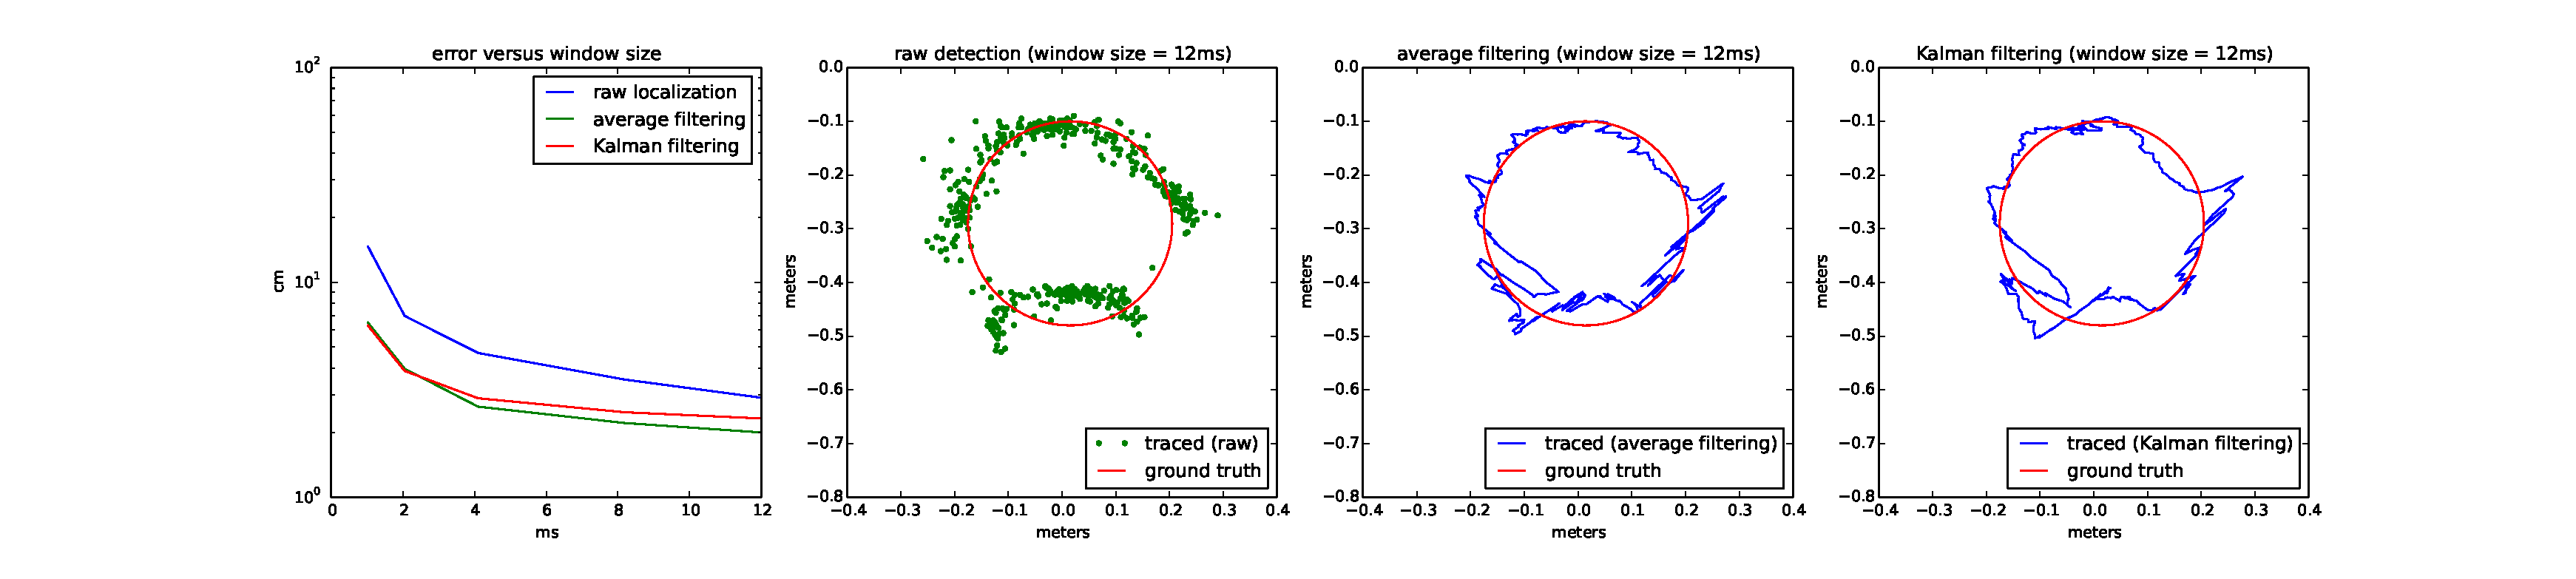
\includegraphics[width=\textwidth]{trace_output_circle_mbn.eps}
  \caption{music B}
  \label{fig:circle_musicbn}
\end{subfigure}
\caption{Localization of circle movement with different sound sources. Sound source is moving at $10$ cm per second}
\label{fig:circle_normal}
\end{figure*}

\begin{figure*}[]
\centering
\begin{subfigure}[]{1.0\textwidth}
  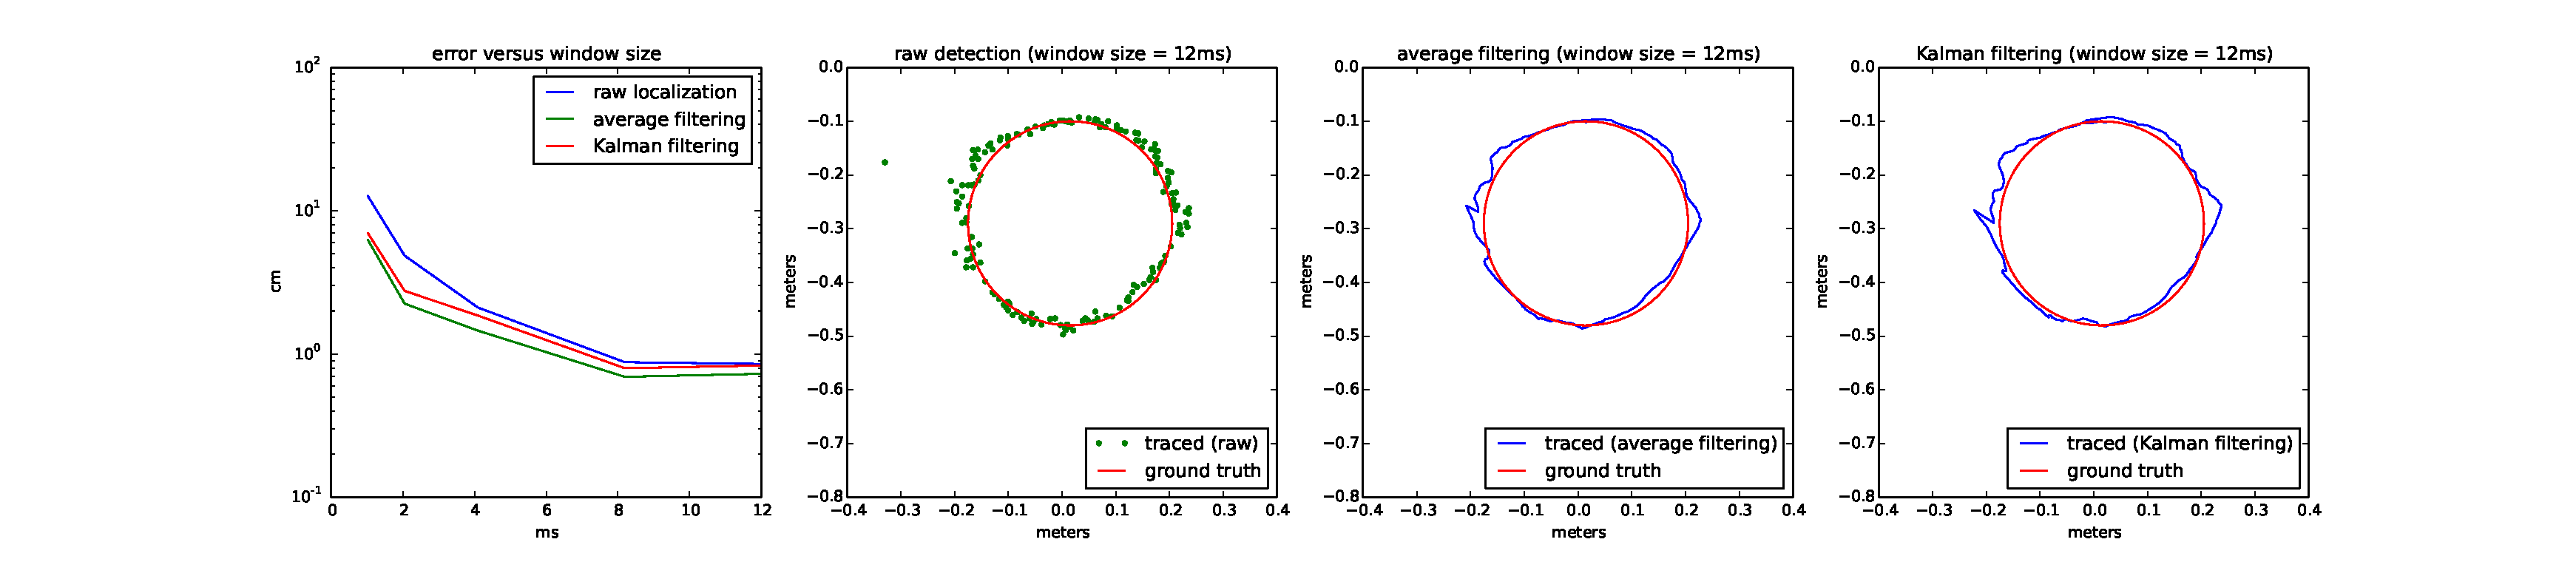
\includegraphics[width=\textwidth]{trace_output_circle_wnf.eps}
  \caption{white noise}
  \label{fig:circle_wnf}
\end{subfigure}
\begin{subfigure}[]{1.0\textwidth}
  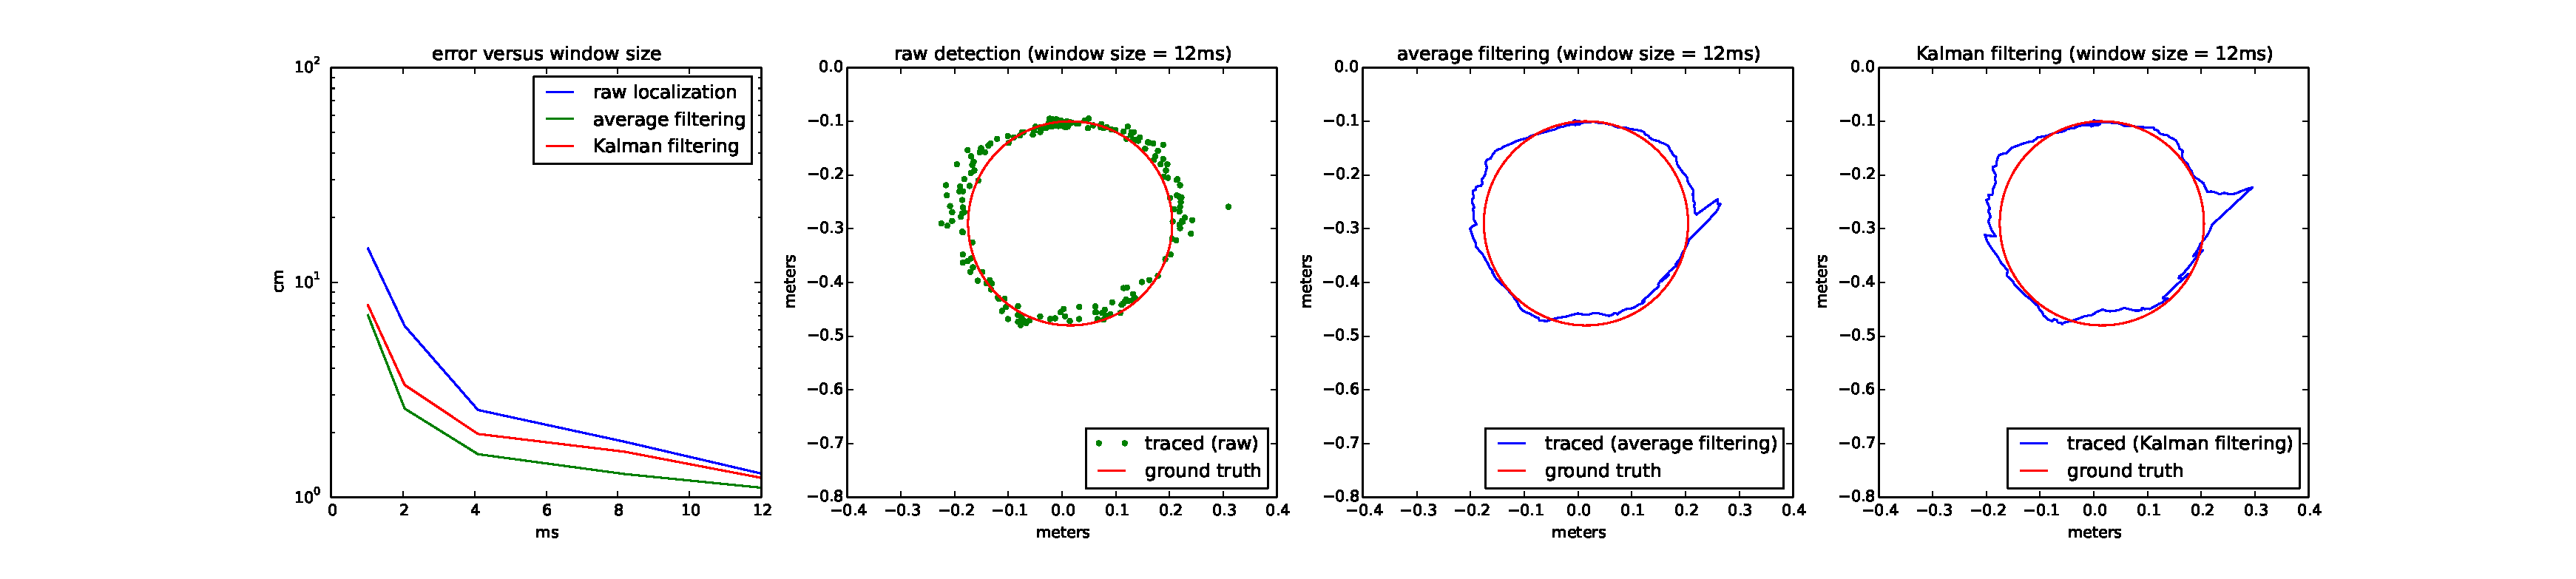
\includegraphics[width=\textwidth]{trace_output_circle_maf.eps}
  \caption{music A}
  \label{fig:circle_musicaf}
\end{subfigure}
\begin{subfigure}[]{1.0\textwidth}
  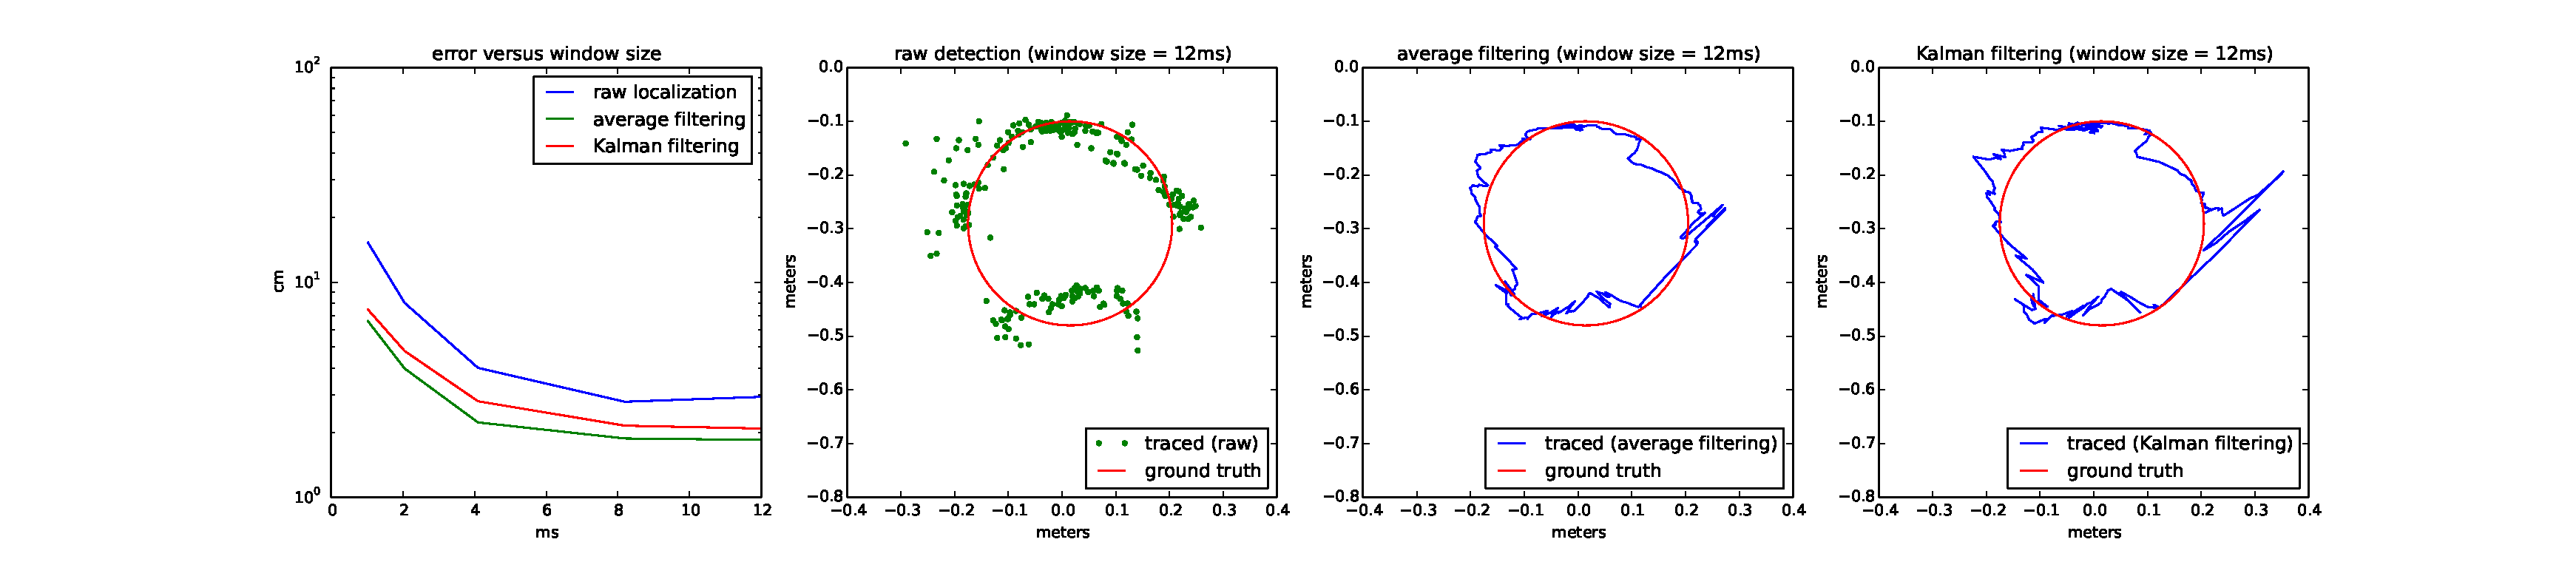
\includegraphics[width=\textwidth]{trace_output_circle_mbf.eps}
  \caption{music B}
  \label{fig:circle_musicbf}
\end{subfigure}
\caption{Localization of circle movement with different sound sources. Sound source is moving at $20$ cm per second}
\label{fig:circle_fast}
\end{figure*}

Fig~\ref{fig:circle_normal} shows results for experiments with at normal speed, and Fig~\ref{fig:circle_fast} shows results at fast speed. By comparing localization error for each audio source between normal movement speed and fast movement speed, we find the localization error does not depend on how fast the sound sorce is moving. For example fig~\ref{fig:circle_musican} and fig~\ref{fig:circle_musicaf} shows that localization error is $1.289$ cm at normal movement speed and $1.291$ cm at fast movement speed.

From fig~\ref{fig:circle_normal}, localization error is $0.9$ cm for white noise, $1.29$ cm for Music A, and $2.9$ cm for Music B. Localization accuracy is the best for white noise source, and worst for Music B. This is consistent with our expectation because low amplitude regions in Music B would cause arrays to lose track of where the source is. This can also be seen from the "blank" regions in fig~\ref{fig:circle_musicbn}.

Fig ~\ref{fig:circle_normal} also shows that raw detection has the most amount of jiggling. Kalman filter reduces the amount of jiggling from raw detection. Averaging filter has the least amount of jiggling. However, averaging filter averages detection outputs from past 0.5 seconds, which makes the filtered output lag the real movement. 
